\documentclass[11pt]{article}
\usepackage{layout}

\usepackage[top=3cm, bottom=3cm, left=4cm, right=2cm]{geometry}

\usepackage{amsmath}
\usepackage{amssymb}
\usepackage{mathrsfs}
\usepackage{amsthm}
\usepackage[utf8]{inputenc}
%\usepackage[latin1]{inputenc} 
\usepackage[T1]{fontenc}  
\usepackage[french]{babel}
\usepackage{titlesec}
\usepackage[pdftex]{graphicx}
\usepackage{graphics}
\usepackage{float}
\usepackage{bbm}

\begin{document}
\renewcommand{\tablename}{Tableau}
\renewcommand{\figurename}{Illustration}

	\begin{titlepage}
		\centering % Centre everything on the title page
		
		\scshape % Use small caps for all text on the title page
		
		\vspace*{7\baselineskip} % White space at the top of the page
		
		%------------------------------------------------
		%	Title
		%------------------------------------------------
		
		\rule{\textwidth}{1.6pt}\vspace*{-\baselineskip}\vspace*{2pt} % Thick horizontal rule
		\rule{\textwidth}{0.4pt} % Thin horizontal rule
		
		\vspace{0.75\baselineskip} % Whitespace above the title
		{\LARGE Estimation des paramètres par la méthode composite \\} % Title
		\vspace{0.75\baselineskip} % Whitespace below the title
		
		\rule{\textwidth}{0.4pt}\vspace*{-\baselineskip}\vspace{3.2pt} % Thin horizontal rule
		\rule{\textwidth}{1.6pt} % Thick horizontal rule
		
		\vspace{3\baselineskip} % Whitespace after the title block
		
		%------------------------------------------------
		%	Subtitle
		%------------------------------------------------
		{\scshape\Large Sous la supervision de \\ Hélène Cossette\\Étienne Marceau\\ } % Editor list
		
		\vspace*{3\baselineskip}
		
		  % Subtitle or further description
		
		\vspace*{3\baselineskip} % Whitespace under the subtitle
		
		%------------------------------------------------
		%	Editor(s)
		%------------------------------------------------
		
		Préparé par
		
		\vspace{0.5\baselineskip} % Whitespace before the editors
		
		{\scshape\Large Alexandre Lepage, \\
			Diamilatou N'diaye, \\} % Editor list
		
		\vspace*{5\baselineskip}
		
		le 03 Juillet 2019
		
		\vspace{0.5\baselineskip} % Whitespace below the editor list
		
		\vfill % Whitespace between editor names and publisher logo
		
		%------------------------------------------------
		%	Publisher
		%------------------------------------------------
		
		
\includegraphics[height=1.2cm]{UL_P.pdf}\\
		
		Faculté des sciences et de génie\\
		École d'actuariat\\
		Université Laval\\     
	\end{titlepage}
	
	%\setcounter{secnumdepth}{0} % sections are level 1
	%\setcounter{section}{1}

\section{Estimation par la Méthode Composite}

	Le but de cette section est d'estimer les paramètres d'une copule archimédienne hiérarchique par la méthode composite. Dans les exemples suivants $N \sim Binom(5,q), \ q=0.2$ et $X \sim Exp(\beta) , \ \beta=1/100$. La copule hiérarchique étudié ici est de loi mère géométrique de paramètre $\alpha_{0}=0.6$ et de loi enfant géométrique de paramètre $\alpha_{1}=0.4$. Les estimations sont réalisées sur un échantillon simulé de $10\,000$ observations.

\section{Première Approche}
	
	La première approche consiste à estimer séparément tous les paramètres. Dans un premier temps, les paramètres $q$ et $\beta$ sont estimés pas les estimateurs du maximum de vraisemblance de leur loi respective. 
	\[ \hat{q} = \frac{\sum^{10\,000}_{i=0} n_{i}}{5\times 10\,000} \]
	\[ \hat{\beta} = \frac{n_{tot}}{\sum^{n_{tot}}_{i=0} X_{i}} \]
	où $n_{tot}$ représente le nombre de $X_{i}$ présents dans l'échantillon.
	
	Ensuite l'estimateur de $\alpha_{0}$ est obtenu en minimisant la fonction de vraisemblance :
	\[ L(\alpha_{0} \vert \hat{q},\hat{\beta}) = (F_{N}(0))^{n_{0}} \prod^{n_{NX}}_{i=1} \left(\frac{\partial}{\partial x} C(F_{N}(n_i),F_{X}(x_i)) - \frac{\partial}{\partial x} C(F_{N}(n_i-1),F_{X}(x_i))\right) \]
	où $n_{NX}$ représente le nombre de couples $(N_{i},X_{i,j})$ présents dans l'échantillon.\\
	
	De plus, avec le modèle collectif du risque définit par $S= \sum_{k=1}^{\infty} X_k \times \mathbbm{1}\{k \leq N\}$, la copule reliant la v.a. $N$ avec n'importe lequel des $X_i$ s'exprime comme
	
	\begin{equation}\label{eq_copule_NX}
		C(u_{0},u_{1}) = \mathscr{L}_{M}(\mathscr{L}_{M}^{-1}(u_{0}) + \mathscr{L}_{M}^{-1}(u_{1}) ).
	\end{equation}

	À noter que la copule décrite en \eqref{eq_copule_NX} est archimédienne.\\
	
	Et enfin, de la même manière que pour $\alpha_{0}$, l'estimateur de $\alpha_{1}$ est obtenu à partir de la fonction de vraisemblance
	
	\[ L(\alpha_{1} \vert\hat{\beta},\hat{\alpha_{0}}) = \prod^{n_{XX}}_{i=0} \frac{\partial^2}{\partial x_{1}\partial x_{2}} C(F_{X}(x_{1}),F_{X}(x_{2}))  \]
	où $n_{XX}$ représente le nombre de couples $\{(X_{i,k},X_{i,j}): k \neq j\}$ présents dans l'échantillon.
	
	\[ C(u_{1},u_{2}) = \mathscr{L}_{\Theta}(\mathscr{L}_{\Theta}^{-1}(u_{1}) + \mathscr{L}_{\Theta}^{-1}(u_{2}) ) \]
	 avec    \[ \mathscr{L}_{\Theta}(t) = \mathscr{L}_{M}(-\ln(\mathscr{L}_{B}(t))) \]
	 et $$ \mathscr{L}^{-1}_{\Theta}(u) = \mathscr{L}_B^{-1}\left(exp(-\mathscr{L}^{-1}_M(u)) \right). $$
	
	Le tableau \ref{resultats_app1} présente les valeurs des estimateurs;
	
	\begin{table}[H]
		\centering
		\begin{tabular}{lrrrr}
			  \hline
			 & $q$ & $\beta$ & $\alpha_{0}$ & $\alpha_{1}$ \\ 
			  \hline
			  Valeur & 0.2000 & 0.0100 & 0.6000 & 0.4000 \\ 
			  Estimateur & 0.1996 & 0.0087 & 0.3603 & 0.8545 \\ 
			  Temps & 0.0000 & 0.0000 & 1.3900 & 0.7900 \\ 
			   \hline
		\end{tabular}
 		\caption{Valeurs estimées de $q$, $\beta$, $\alpha_{0}$, $\alpha_{1}$ ainsi que le temps de calcul par la première approche.}
	 	\label{resultats_app1}
	\end{table}

	On voit en regardant le tableau \ref{resultats_app1} que les résultats de l'estimation sont loins des vrais paramètres.\\

	%Cependant, si on estime $\hat{\beta}$ en ne prenant pas tous les $X_{i,j}$ simultanément dans la maximisation de la vraisemblance, mais que, plutôt, on sélectionne un $X_{i}$ parmi les $X_{i,j}$ de façon aléatoire et que l'on répète cet exercice 100 fois pour créer un vecteur de dimension $10\,000 \times 100$. Alors, d'une part, on obtient un meilleur estimateur pour $\beta$, mais en plus, on augmente la précision pour $\hat{\alpha}_{0}$ comme l'illustre le tableau \ref{tbl_resultats_app1_2}

\subsection{Comportement Asympotique}

	La méthode précédente est répétée 100 fois afin d'observer le comportement asymptotique des estimateurs.
	Pour $\alpha_{0}$,  on obtient une moyenne de 0.3556106 et un intervalle de confiance de niveau $ \alpha = 95\% $ de $[0.3117377,0.3994836]$.
	
	\begin{figure}[H]
		\centering
		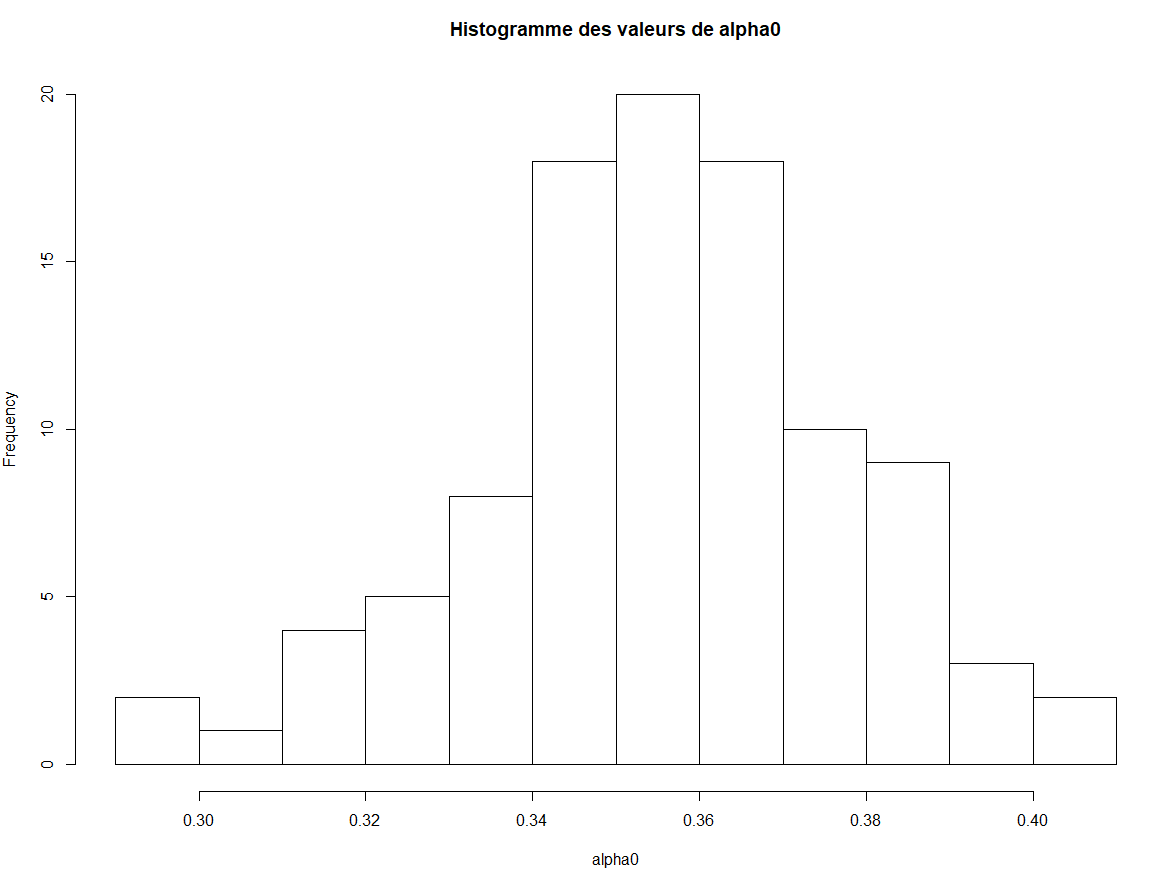
\includegraphics[height=6cm]{alpha0.png}
		\caption[Paramètre $\alpha_{0}$]{Histogramme des valeurs prises par $\alpha_{0}$ sur 100 répétitions} 
		\label{alpha0}
	\end{figure}
		
	Pour $\alpha_{1}$ on obtient une moyenne de  0.8201792 et un intervalle de confiance de niveau $\alpha = 95\% $ de $[0.7704843,0.8698740]$.

	\begin{figure}[H]
		\centering
		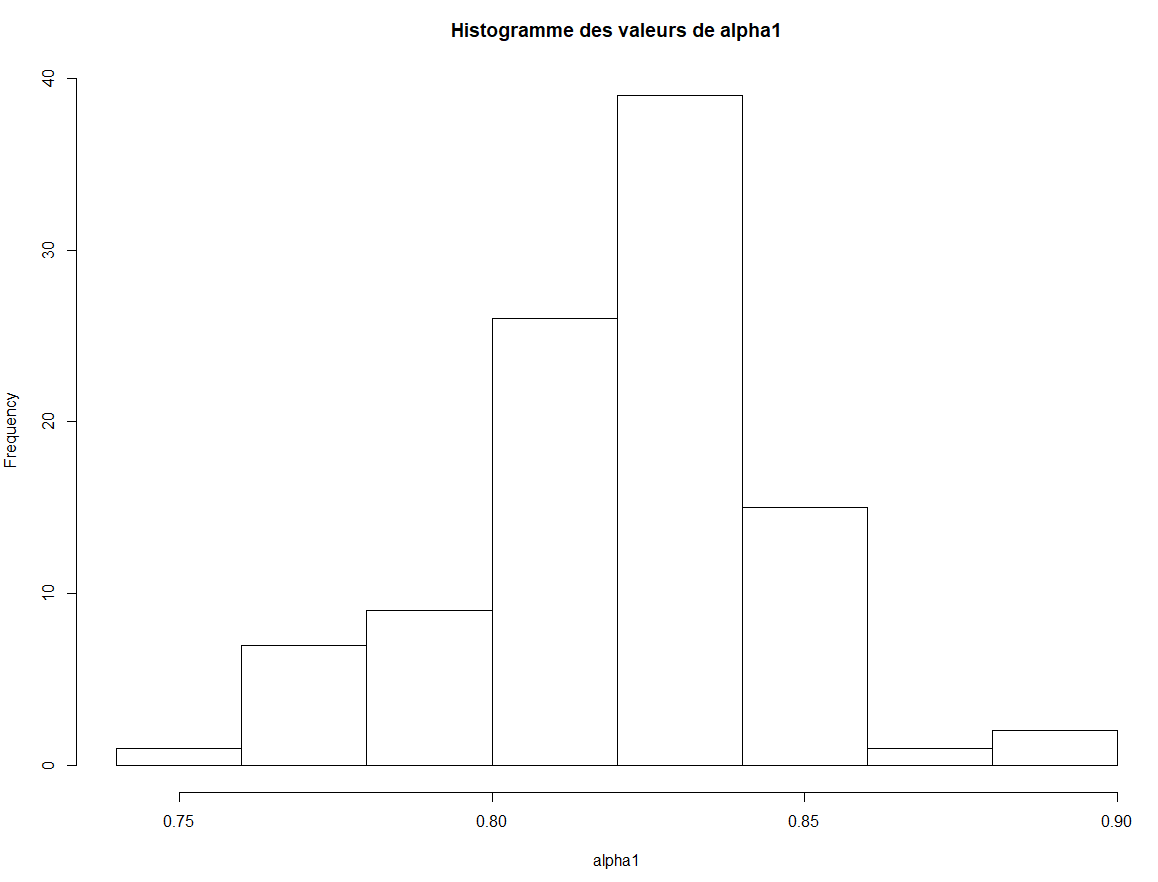
\includegraphics[height=6cm]{alpha1.png}
		\caption[Paramètre $\alpha_{1}$]{Histogramme des valeurs prises par $\alpha_{1}$ sur 100 répétitions} 
		\label{alpha1}
	\end{figure}
		

\subsubsection{Comportement asymptotique des estimateurs pour une copule archimédienne hiérarchique Logarithmique-Gamma de paramètres $(\alpha_{0}=6,\alpha_{1}=4)$}

	L'estimateur de $\alpha_{0}$ produit une moyenne de 3.232702 et un intervalle de confiance de niveau $ \alpha = 95\% $ de $[3.114684,3.350721]$.
	
	\begin{figure}[H]
		\centering
		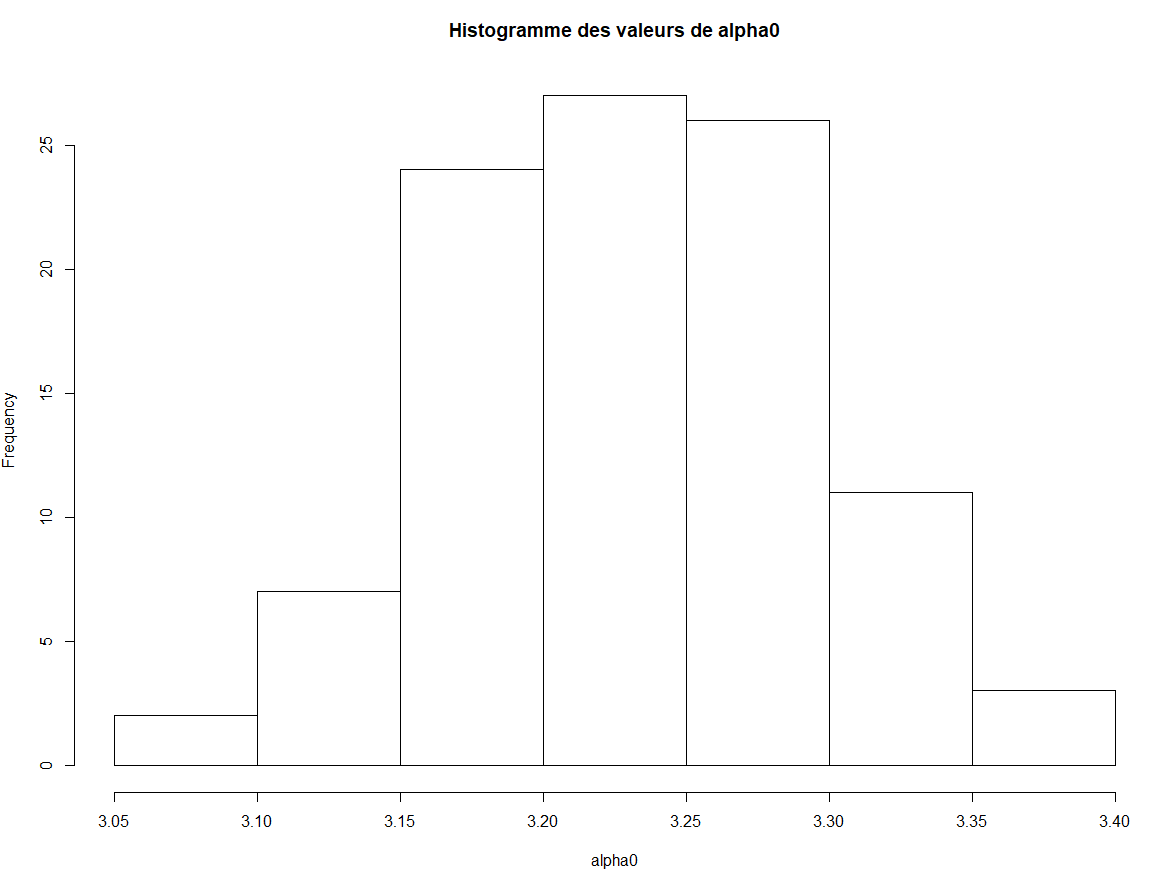
\includegraphics[height=6cm]{alpha0lg.png}
		\caption[Paramètre $\alpha_{0}$]{Histogramme des valeurs prises par $\alpha_{0}$ sur 100 répétitions} 
		\label{alpha0lg}
	\end{figure}
		
	L'estimateur de $\alpha_{1}$ produit  une moyenne de  6.646969 et un intervalle de confiance de niveau $\alpha = 95\% $ de $[6.094799,7.199139]$.

	\begin{figure}[H]
		\centering
		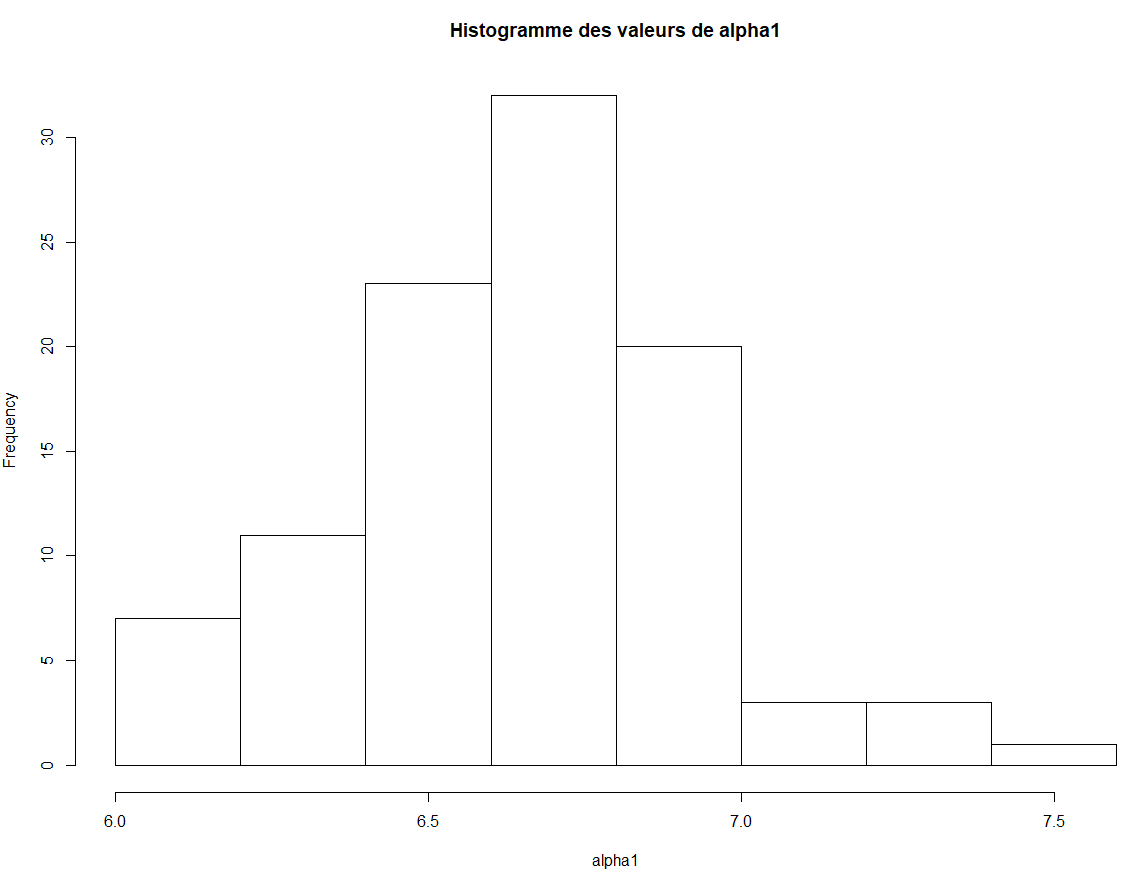
\includegraphics[height=6cm]{alpha1lg.png}
		\caption[Paramètre $\alpha_{1}$]{Histogramme des valeurs prises par $\alpha_{1}$ sur 100 répétitions} 
		\label{alpha1lg}
	\end{figure}
		
	Les estimations sont donc assez loin des vrais paramètres. 

\section{Seconde Approche}

	La seconde approche consiste à estimer $q$, $\beta$ et $\alpha_{0}$ en même temps puis $\alpha_{1}$ par la suite. 
	La fonction de vraisemblance à minimiser est :
	
	
	\[ L(\alpha_{0},q,\beta) = (F_{N}(0))^{n_{0}} \prod^{n_{NX}}_{i=0} \left(\frac{\partial}{\partial x} C(F_{N}(n),F_{X}(x)) - \frac{\partial}{\partial x} C(F_{N}(n-1),F_{X}(x))\right) \]
	où $n_{NX}$ représente le nombre de couples $(N_{i},X_{i,j})$ présents dans l'échantillon.
	\[ C(u_{0},u_{1}) = \mathscr{L}_{M}(\mathscr{L}_{M}^{-1}(u_{0}) + \mathscr{L}_{M}^{-1}(u_{1}) ) \]
	
	Pour ce qui est de $\alpha_{1}$, la même estimation que la section précédente est réalisée.
	
	\[ L(\alpha_{1}\vert \hat{\beta},\hat{\alpha_{0}}) = \prod^{n_{XX}}_{i=0} \frac{\partial^{2}}{\partial x_{1}\partial x_{2}} C(F_{X}(x_{1}),F_{X}(x_{2}))  \]
	\[ C(u_{1},u_{2}) = \mathscr{L}_{\Theta}(\mathscr{L}_{\Theta}^{-1}(u_{1}) + \mathscr{L}_{\Theta}^{-1}(u_{2}) ) \]
	 avec    \[ \mathscr{L}_{\Theta}(t) = \mathscr{L}_{M}(-\ln(\mathscr{L}_{B}(t))) \]
	où $n_{XX}$ représente le nombre de couples $(X_{i,k},X_{i,j})$ présents dans l'échantillon

	Le tableau \ref{resultats_app1} présente les valeurs des estimateurs;

	\begin{table}[H]
		\centering
		\begin{tabular}{rrrrr}
		  \hline
		 	& $q$ & $\beta$ & $\alpha_{0}$ & $\alpha_{1}$ \\  
		  \hline
			Valeur & 0.2000 & 0.0100 & 0.6000 & 0.4000 \\ 
			Estimateur & 0.3589 & 0.0087 & 0.4972 & 0.8000 \\ 
			Temps & 45.6000 & 45.6000 & 45.6000 & 1.4100 \\ 
		   \hline
		\end{tabular}
	 		\caption{Valeurs estimées de $q$, $\beta$, $\alpha_{0}$, $\alpha_{1}$ ainsi que le temps de calcul par la deuxième approche. Le temps de calcul de $q$, $\beta$ et $\alpha_{0}$ est leur temps de calcul commun étant donné qu'ils sont estimés ensembles.}
	 	\label{resultats_app2}
	\end{table}

	Dans le tableau \ref{resultats_app2}, on voit que le niveau de précision est légèrement meilleur que pour la première approche lorsque l'on regarde $\alpha_{0}$ et $\alpha_{1}$, bien que ce ne soit toujours pas satisfaisant. Tandis que pour $\hat{q}$, les résultats se détériorent.

\subsection{Comportement Asympotique}

	L'estimation est ensuite répétée 100 fois afin d'observer le comportement asymptotique des estimateurs.
	L'estimateur de $\alpha_{0}$ produit une moyenne de 0.4856781 et un intervalle de confiance de niveau $\alpha = 95\%$ de $[0.3888275,0.5825286]$.
	
	\begin{figure}[H]
		\centering
		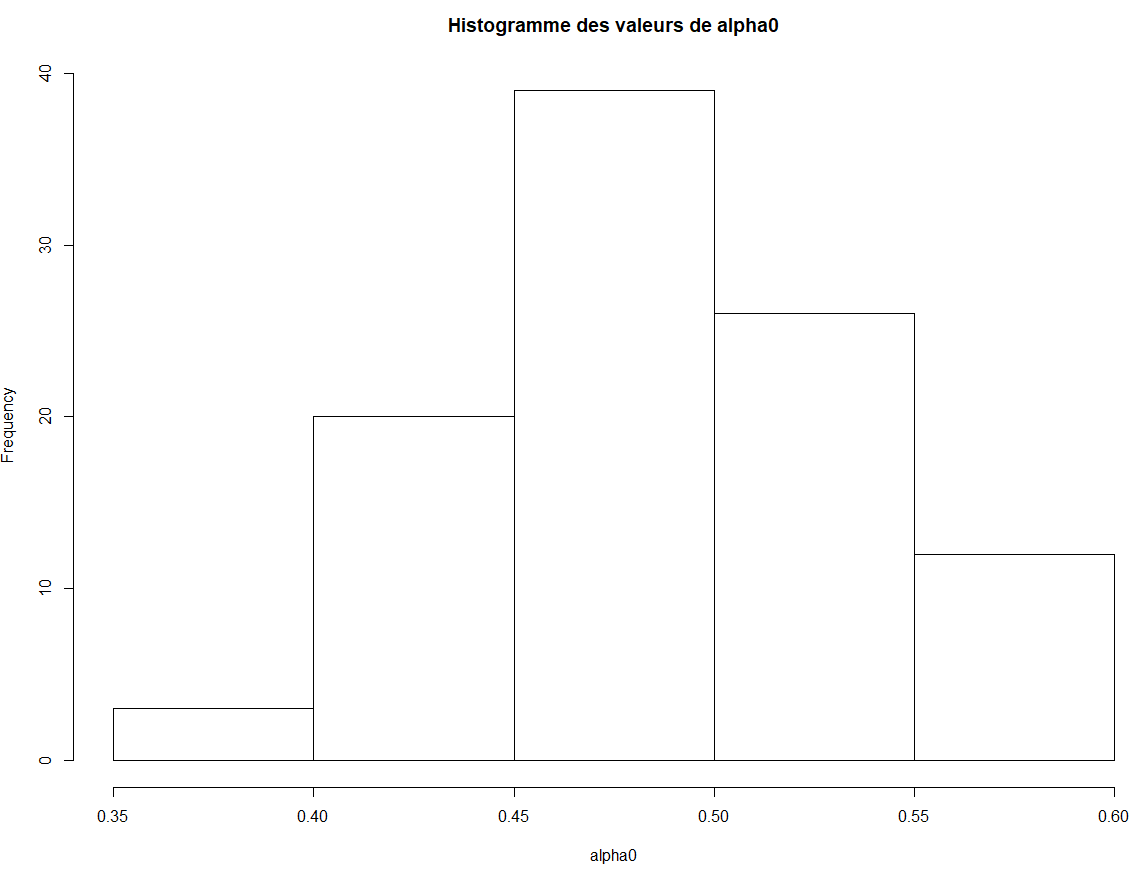
\includegraphics[height=6cm]{alpha02.png}
		\caption[Paramètre $\alpha_{0}$]{Histogramme des valeurs prises par $\alpha_{0}$ sur 100 répétitions} 
		\label{alpha02}
	\end{figure}
		
	L'estimateur de $\alpha_{1}$ produit une moyenne de  0.7690707 et un intervalle de confiance de niveau $\alpha = 95\%$ de $[0.7103108,0.8278306]$.

	\begin{figure}[H]
		\centering
		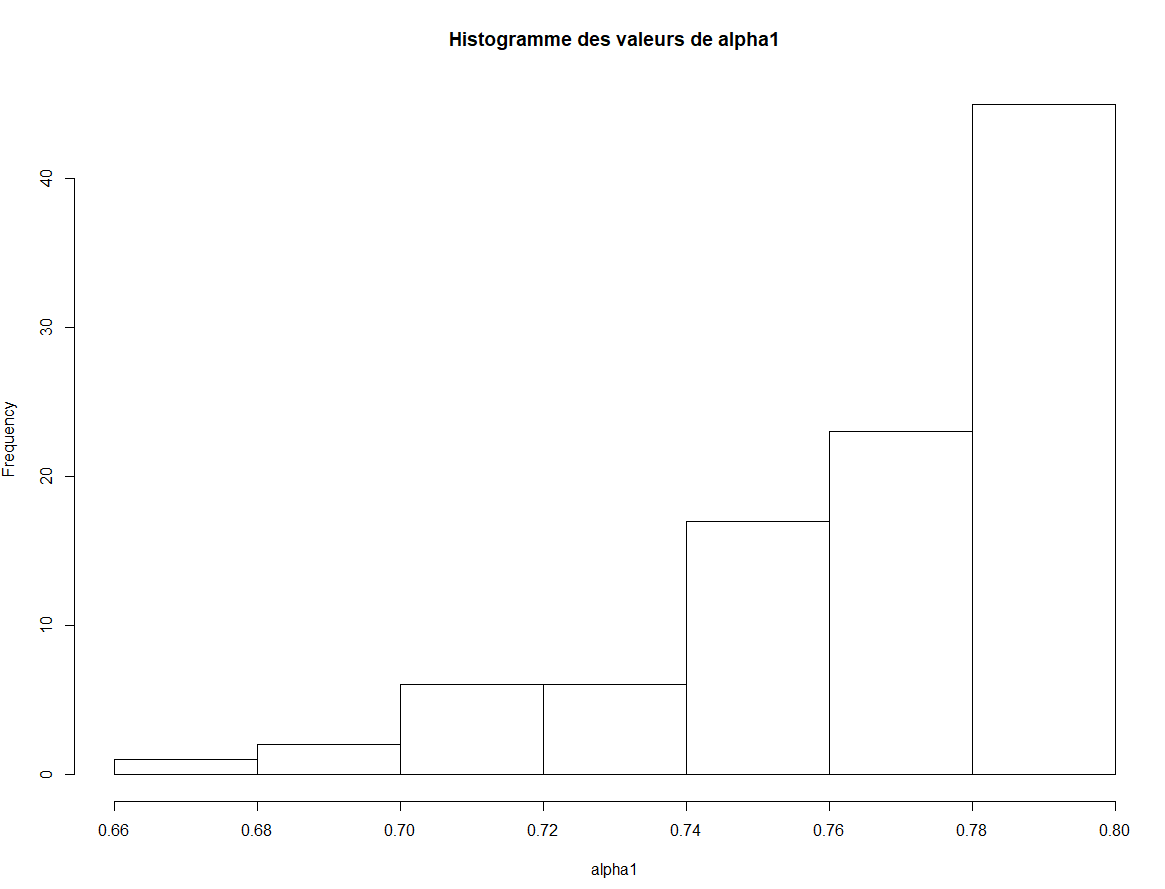
\includegraphics[height=6cm]{alpha12.png}
		\caption[Paramètre $\alpha_{1}$]{Histogramme des valeurs prises par $\alpha_{1}$ sur 100 répétitions} 
		\label{alpha12}
	\end{figure}
		
\end{document}